\chapter{Tool Design}
\label{chap:tool-design}

While GumTree deduces a short edit script between two files and commits itself to present those edit actions at AST level visually, and leave the interpretation of the underlying intents to humans, the goal of this tool \textit{ccdetector} is to further analyze the edit script and identify change intents at a higher level.

\section{Identifiable Changes}

\subsection{Classification Explanation}

\begin{itemize}
	\item \textbf{Function Changes}
	\begin{enumerate}
		\item \textbf{Function Renaming} As previously mentioned, leading underscores in Python function names serve the role as an access modifier. Functions with a leading underscore in its name are \textit{weakly private}, and those without one are \textit{public}.
		\begin{enumerate}
			\item \textbf{Private to Public} The renaming action removes the leading underscores in the function name.
			\item \textbf{Public to Private} The renaming action adds leading underscores in the function name.
			\item \textbf{No Accessibility Switch} The renaming action does not alter the leading underscores if any in the function name.
		\end{enumerate}
		\item \textbf{Function Relocation} Moving a function to a new position in the same file, or to another file.
	\end{enumerate}

	\item \textbf{Parameter Changes}
	\begin{enumerate}
		\item \textbf{Parameter Insertion} Inserting new parameters into the function signature, this action could be affiliated with parameter default value addition.
		\item \textbf{Parameter Removal} Removing existing parameters in the function signature, this action could be affiliated with parameter default value removal.
		\item \textbf{Parameter Update} Renaming existing parameters in function the signature. For a class method, the first parameter usually picks up from \textit{cls} and \textit{self}. \textit{cls} indicates a static method which could be invoked without first instantiating an instance; \textit{self} indicates an instance method that must be invoked by a class instance.
		\begin{enumerate}
			\item \textbf{\textit{cls}/\textit{self} Switch} Switching the first parameter between \textit{cls} and \textit{self}.
			\item \textbf{Normal Update} Renaming a function parameter. Renaming a civilian parameter to \textit{cls}/\textit{self} or the other way round are not commonly observed as possessing \textit{cls}/\textit{self} as parameter or not distinguishes class methods from functions outside any classes. And relocating them would results in inserting or removing a \textit{cls}/\textit{self} parameter rather than updating the first parameter.
		\end{enumerate}
	\end{enumerate}

	\item \textbf{Parameter Default Value Changes}
	\begin{enumerate}
		\item \textbf{Parameter Default Value Addition} Adding default value to a parameter in the function signature.
		\item \textbf{Parameter Default Value Removal} Removing existing default value of a parameter in the function signature.
		\item \textbf{Parameter Default Value Update} Replacing the existing default value of a parameter in the function signature with a new one. Although whether or not the data type of the parameter default value changes does not classifies them into two categories in the outcome, it does effects its detection, which would be explained in detail in the latter sections.
		\begin{itemize}
			\item Same data type
			\item Different data type
		\end{itemize}
	\end{enumerate}

	\item \textbf{Return Type}
	\begin{enumerate}
		\item \textbf{Return Type Addition} Adding a return annotation in the function signature.
		\item \textbf{Return Type Removal} Removing existing return annotation from the function signature.
		\item \textbf{Return Type Update} Replacing existing return annotation with another one.
	\end{enumerate}
\end{itemize}

\subsection{Object-Oriented Programming Class Design}

In this subsection I will explain the class code structure design in the implementation of ccdetector.

\newpage

\begin{figure*}
	\label{fig:ccdetector-class-design}
	\caption{ccdetector class structure design}
	\begin{tikzpicture}
		\begin{class}[text width=7cm]{FunctionRenaming}{0,0}
			\attribute{- oldFunctionName: String}
			\attribute{- newFunctionName: String}
			\attribute{- weaklyPrivate: boolean}
			\attribute{+ Type: enum}
			\operation{+ toString()}
		\end{class}

		\begin{class}[text width=7cm]{ParameterChange}{7.5,0}
			\attribute{- targetFunctionName: String}
			\attribute{- oldParameterName: String}
			\attribute{- newParameterName: String}
			\attribute{+ Type: enum}
			\operation{+ toString()}
		\end{class}

		\begin{class}[text width=7cm]{ParameterDefaultValueChange}{0,-4}
			\attribute{- targetFunctionName: String}
			\attribute{- targetParameterName: String}
			\attribute{- oldParameterName: String}
			\attribute{- newParameterName: String}
			\attribute{+ Type: enum}
			\operation{+ toString()}
		\end{class}

		\begin{class}[text width=7cm]{ReturnTypeChange}{7.5,-4}
			\attribute{- targetFunctionName: String}
			\attribute{- oldReturnTypeName: String}
			\attribute{- newReturnTypeName: String}
			\attribute{+ Type: enum}
			\operation{+ toString()}
		\end{class}
	\end{tikzpicture}
\end{figure*}

\section{Edit Script Generation}

The edit scripts of input Python source files are generated by directly calling GumTree APIs.

\section{Change Detections}

As explained in \hyperref[chap:background]{Background}, edit actions are operations that modify the nodes or subtrees of the AST of the older file. Each edit action object in GumTree API bonds with an AST node (subtree roots for operations on subtrees). The basic idea is to traverse through the edit script produced by GumTree and inspect each edit action along with its corresponding AST node within that edit script and find the ones that match the characteristics of our identifiable changes.

A major concern is the sequential order in which we detect the four general categories of changes. As demonstrated in the skeleton algorithm, I start from changes of a larger scale gradually to smaller scales (\hyperref[fig:change-detect-routine]{Figure 4.2}). Due to the fact that it requires method information to describe a parameter or return type change, and method and parameter information to describe a parameter default value change, Collecting method and parameter change records in advance makes it possible to check if the method or parameter whose default value changed has been renamed.

\tikzstyle{block} = [rectangle, draw, text width=20em, text centered, rounded corners, minimum height=4em]
\tikzstyle{line} = [draw, very thick, -latex']
\tikzstyle{cloud} = [ellipse, draw, text width=6em, node distance=2.5cm, minimum height=2em]

% TODO: Change this figure to ppt version
\begin{figure}
	\caption{Change detection routine}
	\label{fig:change-detect-routine}
	\begin{center}
		\begin{tikzpicture}[scale=2, node distance = 2cm, auto]
			% Place nodes
			\node[block](compute){Compute edit script};
			\node[block, below of=compute](check-func-rename){Check function renaming};
			\node[block, below of=check-func-rename](check-func-relocate){Check function relocation};
			\node[block, below of=check-func-relocate](check-param){Check parameter changes};
			\node[block, below of=check-param](check-param-default-val){Check parameter default value changes};
			\node[block, below of=check-param-default-val](check-return){Check return type changes};
			% Draw edges
			\path[line](compute) -- (check-func-rename);
			\path[line](check-func-rename) -- (check-func-relocate);
			\path[line](check-func-relocate) -- (check-param);
			\path[line](check-param) -- (check-param-default-val);
			\path[line](check-param-default-val) -- (check-return);
		\end{tikzpicture}
	\end{center}
\end{figure}

\begin{figure}
	\caption{Typical AST structure of a function signature}
	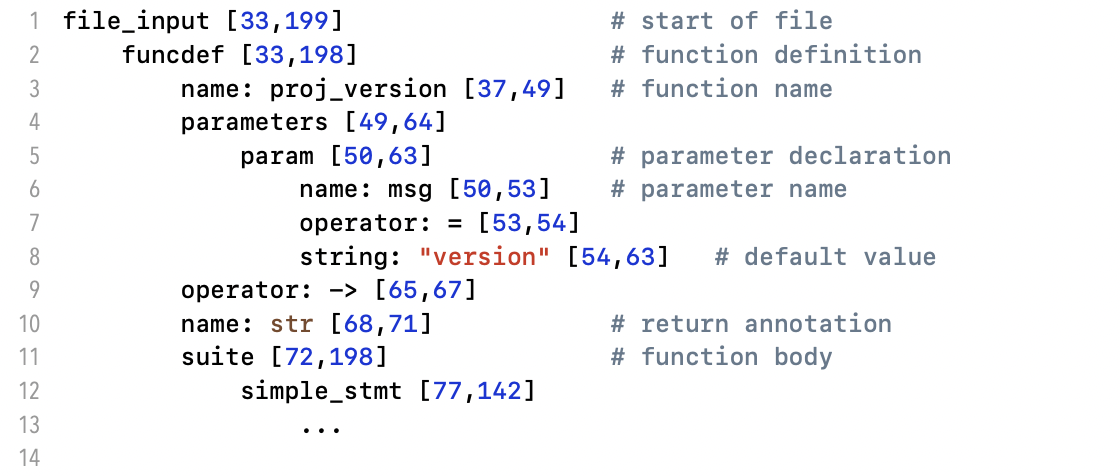
\includegraphics[width=\textwidth]{ast.png}
\end{figure}

\subsection{Function Renaming Detection}
\label{subsec:func-rename-detect}

Function renaming changes are recorded in an \textit{Update} action that changes the label of the first child \textit{name} node of \textit{funcdef} node, this is to be distinguished from return annotation updates which affects the fourth child \textit{name} node of \textit{funcdef}. After locating a function renaming operation, inspecting leading underscores in the old function name as well as the new one determines the accessibility modification status.

\begin{algorithm}
	\label{algo:function-renaming-detection}
	\caption{Function renaming detection algorithm}
	\SetAlgoLined
	\begin{algorithmic}[1]
		\REQUIRE Edit script $S$ and collection of function renaming changes $R$
		\FORALL{$A \in S$}
			\STATE $node \gets$ getNode($A$);
			\IF{$A \in$ Update \\
			\AND $node \in$ name \\
			\AND getParent($node$) $\in$ funcdef \\
			\AND posInParent($node$) $= 0$}
				\STATE $old \gets$ getLabel($node$);
				\STATE $new \gets$ getValue($A$);
				\IF{$old$.startsWith("$\_$") \AND $!new$.startsWith("$\_$")}
					\STATE $record \gets$ renaming (private to public);
				\ELSIF{$new$.startsWith("$\_$") \AND $!old$.startsWith("$\_$")}
					\STATE $record \gets$ renaming (public to private);
				\ELSE
					\STATE $record \gets$ renaming (no accessibility switch);
				\ENDIF
				\STATE Append $record$ to $R$;
			\ENDIF
		\ENDFOR
	\end{algorithmic}
\end{algorithm}

\subsection{Parameter Change Detection}
\label{subsec:param-change-detect}

Parameter changes include \textit{Parameter Insertion}, \textit{Parameter Removal}, \textit{Parameter Normal Update}, and \textit{cls/self Switch}. A parameter change record in ccdetector's output includes the name of the function whose parameter changed, the old and renewed parameter names, and the specific change type (\hyperref[fig:ccdetector-class-design]{Figure 4.1}).

Python supports many kinds of special parameters other than normal ones, in Python 3 it introduced the \textit{* (a bare asterisk)} operator to be placed among parameters (\hyperref[lst:asterisk-op]{Figure 4.4}), indicating that all parameters before this asterisk require positional arguments, while all parameters after it require keyword arguments.

\begin{figure}[!t]
	\lstinputlisting[
		language=diff,
		caption={Bare asterisk operator \& None default value},
		label={lst:asterisk-op}
	]{code_snippets/asterisk_operator.diff}
	\vspace{-5mm}
\end{figure}

\begin{enumerate}
	\item \textbf{Parameter Insertion/Removal} Normally, these records are stored in \textit{TreeInsert} and \textit{TreeDelete} actions that operate on a subtree rooted at a \textit{param} node. In the special scenarios of inserting or deleting an \textit{*} operator in the function signature, the edit script generated by GumTree would store an \textit{Insert}/\textit{Delete} action that deals with a single \textit{operator} node under the \textit{parameters} parent.
	\item \textbf{Parameter Update} This kind of changes are indicated by an \textit{Update} action that changes the label of the child \textit{name} node under \textit{param} parent. Further investigations of whether the two involved names are cls and self will decide that this update is a normal one or a cls/self switch.
\end{enumerate}

ccdetector automatically checks if the target function of a parameter change operation has been renamed in the findings of \hyperref[subsec:func-rename-detect]{Function Renaming Detection}, and record the current name of the target function.

\begin{algorithm}
	\label{algo:parameter-change-detection}
	\caption{Parameter change detection algorithm}
	\begin{algorithmic}[1]
		\REQUIRE Edit script $S$ and collection of parameter changes $R$
		\FORALL{$A \in S$}
			\STATE $node \gets$ getNode($A$);
			\IF{$A \in$ TreeInsert
			\AND $node \in$ param}
				\STATE $record \gets$ parameter insertion;
			\ELSIF{$A \in$ TreeDelete
			\AND $node \in$ param}
				\STATE $record \gets$ parameter removal;
			\ELSIF{$A \in$ Insert
			\AND getParent($node$) $\in$ parameters \\
			\AND $node \in$ operator
			\AND getLabel($node$) $= *$}
				\STATE $record \gets$ parameter insertion;
			\ELSIF{$A \in$ Delete
			\AND getParent($node$) $\in$ parameters \\
			\AND $node \in$ operator
			\AND getLabel($node$) $= *$}
				\STATE $record \gets$ parameter removal;
			\ELSIF{$A \in$ Update}
				\STATE $old \gets$ getLabel($node$);
				\STATE $new \gets$ getValue($A$);
			\IF{$old =$ cls \AND $new =$ self \OR \\
				$old =$ self \AND $new =$ cls}
					\STATE $record \gets$ cls/self switch;
				\ELSE
					\STATE $record \gets$ normal update;
				\ENDIF
			\ENDIF
			\STATE Append $record$ to $R$;
		\ENDFOR
	\end{algorithmic}
\end{algorithm}

\subsection{Parameter Default Value Change Detection}

Parameter default value changes include \textit{Parameter Default Value Addition}, \textit{Parameter Default Value Removal}, and \textit{Parameter Default Value Update}. The data types of the default values are generally divided into three categories:

\begin{itemize}
	\item \textbf{Primitive types} Strings and numeric data types are stored in single AST nodes, relating to Insert, Delete, and Update edit actions.
	\item \textbf{\textit{Lists}, \textit{Dictionaries}, and container types} These values are represented as subtrees rooted at an \textit{atom} node. Addition, removal, and even update operations on these values usually involve tree edit actions TreeInsert and TreeDelete.
	\item \textbf{\textit{None}} The \textit{None} default value is worth additional attention as there are no AST nodes defined for it by GumTree's parser. Modifications related to it are still traceable though, as Update actions operate on existing AST nodes, and the addition and removal of default value nodes always occur alongside the same operation of the delimiter (an \textit{operator} node whose label is a comma symbol) before them. So adding or removing a comma operator under a param parent would be regarded as adding or removing a \textit{None} default value, and adding or removing a comma operator following a value node would be regarded as adding or removing a normal default value.
\end{itemize}

A parameter default value change record's attributes contain the names of the function and parameter locating the spot of the changed default value, the previous and current value stored in strings, as well as the specific subdivided change category (\hyperref[fig:ccdetector-class-design]{Figure 4.1}).

\begin{enumerate}
	\item \textbf{Parameter Default Value Addition/Removal} These changes are usually stored in a \textit{Insert}/\textit{Delete} action that adds or removes a single child node of \textit{param} nodes, but there are some special cases to be considered:
	\begin{enumerate}
		\item \textbf{Affilated with parameter insertion/removal} Default values might come and go with their parameters as collateral effects in parameter insertions/removals. Essentially, we could review the parameter insertion/removal records obtained in \hyperref[subsec:param-change-detect]{Parameter Change Detection}, and check if the inserted/removed subtree rooted at a \textit{param} node contains default values.
		\item \textbf{The \textit{None} value}
	\end{enumerate}
	\item \textbf{Parameter Default Value Update} Unlike separating normal parameter updates from cls/self switches, updating a parameter default value with a new value of the same or different data type will not change the subdivided category of the operation. Though they do require different detection techniques.
	\begin{enumerate}
		\item \textbf{Same data type} This will be stored in an \textit{Update} edit action that alters the label of a default value node.
		\item \textbf{Different data type} This will be recorded as two separated edit actions, one removing the obsolete default value node from the AST and one adding the node of the new default value at the same spot. This change cannot be detected in one move because it is impossible to tell a default value addition/removal operation from one of these by inspecting only one action. The only distinguishing factor is that the two actions in this change operate under the same \textit{param} parent node. In the edit script generated by GumTree, \textit{Insert} actions are listed before \textit{Delete} actions. So we collect all the added nodes in Insert actions in a list, and seek for matches when processing the sequence of Delete actions in the edit script (\hyperref[algo:check-param-update-remove]{Algorithm 4.4}). On finding a matched pair of nodes of Insert and Delete actions, add a default value update to the records, otherwise, we have found a default value removal. After exhausting actions in the edit script, the remaining added nodes in the list are of default value addition.
	\end{enumerate}
\end{enumerate}

\begin{algorithm}
	\caption{Parameter default value change detection algorithm}
	\begin{algorithmic}[1]
		\REQUIRE Edit script $S$, collection of parameter insertions $I$, collection of parameter deletions $D$, collection of added nodes $A$, collection of removed nodes $M$, and collection of parameter default value changes $R$
		\FORALL{$pi \in I$ $pd \in D$}
			\STATE $node \gets$ getNode($pi$);
			\IF{getChildrenSize($node$) > 2}
				\STATE Add a parameter default value addition record to $R$;
			\ENDIF
			\STATE $node \gets$ getNode($pd$);
			\IF{getChildrenSize($node$) > 2}
				\STATE Add a parameter default value addition record to $R$;
			\ENDIF
		\ENDFOR
		\STATE $addedNodes \gets$ []
		\STATE $removedNodes \gets$ []
		\FORALL{$A \in G$}
			\STATE $node \gets$ getNode($A$);
			\IF{$A \in$ TreeInsert
			\AND getParent($node$) $\in$ param \\
			\AND $node \in$ atom}
				\STATE Add $node$ to $addedNodes$;
			\ELSIF{$A \in$ TreeDelete
			\AND getParent($node$) $\in$ param \\
			\AND $node \in$ atom}
				\STATE checkParameterDefaultValueRemovalUpdate($node$);
			\ELSIF{$A \in$ Insert
			\AND getParent($node$) $\in$ param \\
			\AND $node \in$ (string | number)}
				\STATE Add $node$ to $addedNodes$;
			\ELSIF{$A \in$ Delete
			\AND getParent($node$) $\in$ param \\
			\AND $node \in$ (string | number)}
				\STATE checkParameterDefaultValueRemovalUpdate($node$);
			\ELSIF{$A \in$ Update
			\AND getParent($node$) $\in$ param \\
			\AND getName($node$) = "name"}
				\STATE Add a parameter default value update record to $R$;
			\ENDIF
		\ENDFOR
		\FORALL{$a \in A$}
			\STATE Add a parameter default value addition record to $R$;
		\ENDFOR
		\FORALL{$m \in M$}
			\STATE Add a parameter default value removal record to $R$;
		\ENDFOR
	\end{algorithmic}
\end{algorithm}

\begin{algorithm}
	\caption{Check for parameter default value update/removal}
	\label{algo:check-param-update-remove}
	\begin{algorithmic}[1]
		\REQUIRE Action node $n$, collection of added nodes $A$, collection of removed nodes \\
		$M$, and collection of parameter default value changes $R$
		\STATE $b \gets False$;
		\FORALL{$a \in A$}
			\IF{(getParamName($n$) = getParamName($a$) \\
			\AND getFuncName($n$) = getFuncName($a$)) \\
			\OR getPos($n$) = getPos($a$)}
				\STATE Add a parameter default value update record to $R$;
				\STATE Remove $a$ from $A$;
				\STATE $b$ = $True$;
			\ENDIF
		\ENDFOR
		\IF{$b$ = $False$}
			\STATE Add $n$ to $M$;
		\ENDIF
	\end{algorithmic}
\end{algorithm}

\subsection{Return Type Change Detection}

Return annotations are type hints in the function signature indicating the type of the value returned by the function. Checking for return annotation changes is akin to a simplified process of checking parameter default value changes. The AST node of return annotation is a \textit{name} node under \textit{funcdef} parent, at the same level as \textit{parameters} which is the parent of all parameter (\textit{param}) nodes (\hyperref[algo:return-change-detect]{Algorithm 4.5}). There are generally three types: \textit{Return Type Addition}, \textit{Return Type Removal}, and \textit{Return Type Update}.

\begin{algorithm}
	\caption{Return type change detection algorithm}
	\label{algo:return-change-detect}
	\begin{algorithmic}[1]
		\REQUIRE Edit script $S$, collection of added nodes $A$, collection of removed nodes \\
		$M$, and collection of return type changes $R$
		\FORALL{$A \in S$}
			\STATE $node \gets$ getNode($A$);
			\IF{$node \in$ name
			\AND getParent($node$) $\in$ funcdef \\
			\AND getPosInParent($node$) = 3}
				\IF{$A \in$ Insert}
					\STATE Add a return type addition record to $R$;
				\ELSIF{$A \in$ Delete}
					\STATE Add a return type removal record to $R$;
				\ELSIF{$A \in$ Update}
					\STATE Add a return type update record to $R$;
				\ENDIF
			\ENDIF
		\ENDFOR
	\end{algorithmic}
\end{algorithm}
